\DiaryEntry{Permutations, 2 (Derangements)}{2015-12-26}{Combinatorics}

As stated before, a permutation is a bijection (one-to-one mapping) from $\mathcal{S}$ onto $\mathcal{S}$.

A permutation can have fixed points; these are elements $x^\star$ which stay constant under the mapping: $\sigma(x^\star) = x^\star$. In ``permutation notation'', a fixed point has the following form $(n)$ where $n$ is any element of $\Sc$ (i.e. it is a cycle of length $1$).

The opposite to fixed points are derangements, which are permutations of the elements, such that no element appears in its original position.

If we take $\Sc = \{1,2,3,4\}$, then there are $4!$ permutations. Out of these, the derangements are as follows

\begin{align}
    & (1,4,3,2), (1,2,3,4), (1,3,4,2), (1,3,2,4), (1,2,4,3), (2,1,3,4) \nonumber \\
    & (1,2)(3,4), (1,3)(2,4), (1,4)(2,3)
        \label{2015-12-26:eq1}
\end{align}

In total, there are $9$ derangements. Per definition, there are no fixed points (otherwise it won't be a derangement), and some permutations with $2$-cycles and with $4$-cycles. There are no $3$-cycles, as a $3$-cycle would cause a $1$-cycle which is not allowed; e.g. $(1,2,3)(4)$.

We will denote with $!n$ the number of derangements of $n$ elements; from above example it follows that $!3 = 9$.

\subsubsection{Number of Derangements}

Now, let's count the number of derangements. We consider the permutation of the first position $\sigma(1) = i$ with $i \neq 1$ (otherwise it won't be a fixed point). There are $n-1$ ways to select such an $i$. Next we need to select a value for $\sigma(i)$; i.e. how we chose the next point. There are two options:

\begin{itemize}
    \item We choose any $i \neq 1$ (and $\sigma(i) \neq i$). In this case we have a derangement with $n-1$ elements.
    \item We choose $\sigma(i)=1$; i.e. we create a $2$-cycle $(1,i)$. A derangement with $n-2$ elements remains.
\end{itemize}

These two options are disjoint and we therefore can add the number of cases. Considering that we can select the original $i$ in $n-1$ ways, we obtain for the number of derangements the following recurrence relation,

\begin{equation}
\label{2015-12-26:eq2}
!n = (n-1) \left[ !(n-1) +  !(n-2)\right]
\end{equation}

The initial conditions are $!0=1$ and $!1=0$. The following Figure shows these two cases.

\begin{figure}[H]
    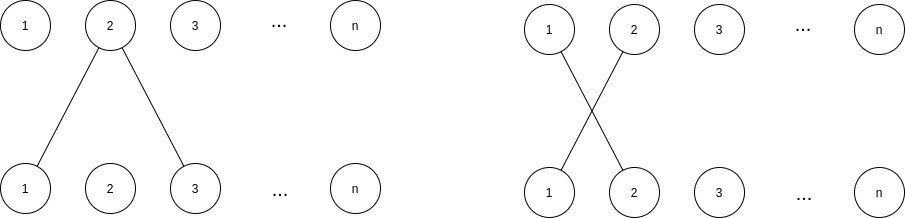
\includegraphics[scale=0.5]{images/2015-12-26-permutations_02_01.png}
\end{figure}

Let's calculate $!n$ for some values of $n$,

\begin{align*}
  &n=2: !2 = 1 [!1 + !0] = 1 [0 + 1] = 1 \\
  &n=3: !3 = 2 [!2 + !1] = 2 [1 + 0] = 2 \\
  &n=4: !4 = 3 [!3 + !2] = 3 [2 + 1] = 9
\end{align*}

for $n=2$, there is only one derangement (which is $(2,1)$) and $!3 = 2$ with the two derangements being $(2,3,1)$ and $(3,1,2)$.

Further values $!n$ are as follows,

\vspace*{2mm}

\begin{tabular}{c|ccccccccccc}
  n &  0 & 1 & 2 & 3 & 4 &  5 &   6 &   7 &     8 & 9 &           10 \\ \hline
  !n & 1 & 0 & 1 & 2 & 9 & 44 & 265 &1854 & 14833 & 133496 & 1334961 \\
\end{tabular}

\vspace*{2mm}

which is \href{https://oeis.org/A000166}{OEIS sequence A000166}.

In the example above with $n=4$, the permutations in the first row of \eqref{2015-12-26:eq1} correspond to case 1, the permutations in the second row of \eqref{2015-12-26:eq1} correspond to case 2 (therefore, they contain $2$-cycles).


\subsubsection{Relation with Factorial}

Other formulas for the number of derangements are (taken from \href{https://en.wikipedia.org/wiki/Derangement}{Wikipedia}),

\bee
!n = n! \sum_{i=0}^n \frac{(-1)^i}{i!}, \quad !n = \left[ \frac{n!}{e} \right] = \left\lfloor \frac{n! + 1}{e} \right\rfloor
\eee

As the factorial counts the number of \emph{all} permutations and not all permutations are derangements, we have $!n < n!$.

We can make this more precise by considering the following limit expression,

\bee
\lim_{n \rightarrow \infty} \frac{!n}{n!} = \lim_{n \rightarrow \infty} n! \sum_{i=0}^n \frac{(-1)^i}{i!} \frac{1}{n!} = \lim_{n \rightarrow \infty} \sum_{i=0}^n \frac{(-1)^i}{i!} = e^{-1} \approx 0.368
\eee

So the number of derangements grows in the same manner as the factorial for large values of $n$. Above expression is also the limit of the probability that a randomly selected permutation of a large number of objects is a derangement. The probability converges to this limit extremely quickly as $n$ increases, which is why $!n$ is the nearest integer to $n!/e$. 


\subsection{Also Interesting...}

We observe that we can express the factorial with the same recurrence relation as \eqref{2015-12-26:eq1},

\begin{equation}
\label{2015-12-26:eq3}
n!= (n-1) \left[ (n-1)! +  (n-2)!\right]
\end{equation}

because

\bee
n(n-1)! - (n-1)! + (n-2)! (n-1) = n! - (n-1)! + (n-1)! = n!
\eee

Some more stuff can be found \href{http://math.ucr.edu/home/baez/qg-winter2004/derangement.pdf}{here}.

%%% Local Variables:
%%% mode: latex
%%% TeX-master: "journal"
%%% End:
